\documentclass[11pt]{article}

\usepackage[margin=1in]{geometry}
\usepackage{amsmath}
\usepackage{amssymb}
\usepackage{booktabs}
\usepackage{graphicx}
\usepackage[hidelinks]{hyperref}
\usepackage[T1]{fontenc}
\usepackage[utf8]{inputenc}
\usepackage{lmodern}
\graphicspath{{../images/}}
\setlength{\emergencystretch}{3em}

\title{Legacy Homogeneous Reactor Study\\[0.4em]
\large One-Group Diffusion and Retired Backends}
\author{}
\date{}

\begin{document}

\maketitle
\tableofcontents
\clearpage

\section{Purpose and status}

This document records the first reactor-physics workflow developed for Reactor
Kinetics Lab.  It covers the homogeneous buckling estimate, the more detailed
one-group annular $r$--$z$ diffusion model, and the two backend services that
were built from it.

These models are \textbf{legacy}.  The frontend no longer exposes the
one-group Core or Transient Diffusion pages.  Current point kinetics uses an
OpenMC continuous-energy rod-worth table, OpenMC-derived delayed-neutron data,
and FMU thermal feedback.  The current Core page uses resolved four-group
diffusion.  Those active models are documented in
\texttt{reactor\_model\_theory.pdf}.

The legacy study remains useful for understanding the numerical development of
the project and the motivation for moving to OpenMC.  It also still supplies
the 20 MW nominal operating scale, the displayed
$1.5\times10^{12}\ \mathrm{n\,cm^{-2}\,s^{-1}}$ flux normalization, and
historical geometry metadata in \texttt{calibration.py}.

\section{First diffusion model and transition to OpenMC}

The original question was whether a heavy-water-moderated, natural-uranium
reactor could be explored with a small, understandable diffusion model.  The
notebook \path{docs/oneGroupHomogeneous.ipynb} answered that question in two
steps:
\begin{enumerate}
  \item a homogeneous bare-cylinder buckling estimate for scale;
  \item a piecewise one-group, two-dimensional annular diffusion solve for
        geometry, leakage, and rod motion.
\end{enumerate}

\begin{figure}[ht]
  \centering
  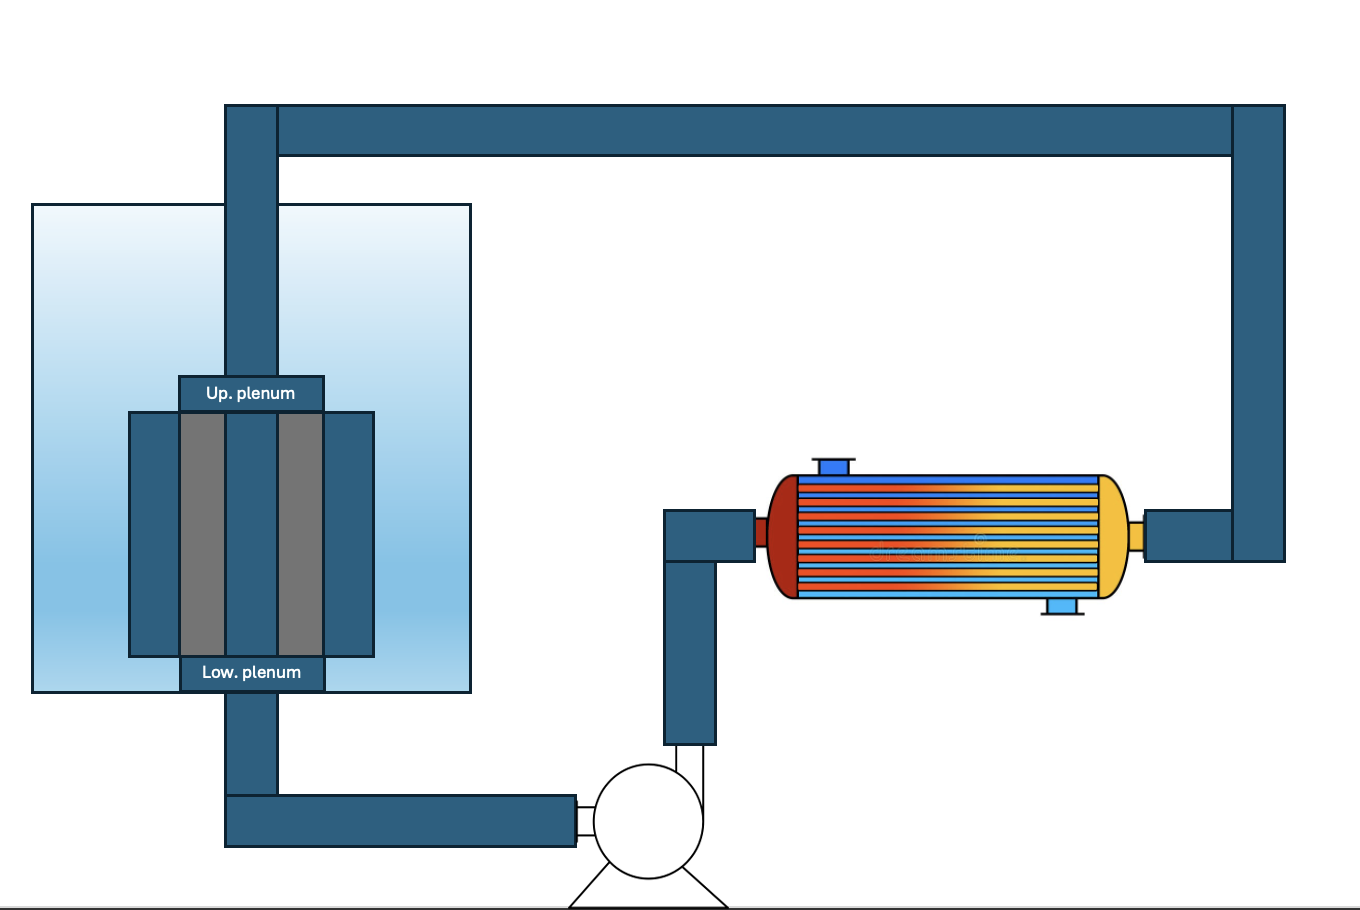
\includegraphics[width=0.84\textwidth]{oldReactorModel.png}
  \caption{The exploratory homogeneous/annular reactor model used before the
  OpenMC reactor was developed.}
\end{figure}

The exercise established the sparse eigenvalue and transient methods later
reused in the project.  It also showed why the reactor definition could not
remain a set of tuned one-group constants.  The effective absorption had to
represent unresolved spectral leakage, the fuel lattice was collapsed into one
annulus, and the rod became an artificial absorbing cylinder.  Because those
choices were coupled, agreement in critical size could not independently
validate material physics or rod worth.  This limitation motivated the
continuous-energy OpenMC model and the tracked reference-data workflow.

\section{Estimate 1: homogeneous buckling}

\subsection{One-speed model}

The first estimate uses one-speed diffusion theory in a homogeneous bare
cylinder:
\[
-D\nabla^2\phi+\Sigma_a\phi
=\frac{1}{k}\nu\Sigma_f\phi.
\]
For a critical homogeneous system, material and geometric buckling satisfy
\[
B_m^2=\frac{\nu\Sigma_f-\Sigma_a}{D}=B_g^2,
\]
with the finite-cylinder approximation
\[
B_g^2\approx
\left(\frac{2.405}{R}\right)^2+\left(\frac{\pi}{H}\right)^2.
\]

The estimate gives a first-pass critical size and checks the direction of
leakage changes.  It cannot represent the central moderator opening, separate
reflector regions, axial reflector slabs, or a moving geometric rod.

\subsection{Homogenization and power amplitude}

Natural uranium and D$_2$O are volume-averaged into one effective core
material.  The criticality equation determines an eigenvalue and shape, not an
absolute amplitude: if $\phi$ is a solution, then $C\phi$ is also a solution.
The notebook therefore obtains a physical flux scale separately from
\[
P=E_f\int_V\Sigma_f(\mathbf r)\phi(\mathbf r)\,dV.
\]

This distinction remains relevant in the current application.  Point kinetics
evolves a normalized neutron population and then applies independent nominal
power and flux scales.

\section{Estimate 2: one-group annular $r$--$z$ model}

\subsection{Geometry}

Estimate 2 solves a heterogeneous one-group diffusion eigenproblem on an
axisymmetric cylindrical mesh:
\[
-\nabla\cdot(D\nabla\phi)+\Sigma_a\phi
=\frac{1}{k_{\mathrm{eff}}}\nu\Sigma_f\phi.
\]
The legacy frozen geometry is:

\begin{center}
\begin{tabular}{lc}
\toprule
Quantity & Value \\
\midrule
Inner moderator radius & $80.0$ cm \\
Fuel outer radius & $345.6$ cm \\
Reflector outer radius & $405.6$ cm \\
Active height & $691.2$ cm \\
Axial reflector thickness & $60.0$ cm per side \\
Equivalent rod radius & $50.0$ cm \\
\bottomrule
\end{tabular}
\end{center}

Only $r\geq0$ is meshed, but cylindrical volume weighting
$2\pi r\,dr\,dz$ represents the complete three-dimensional body.

\subsection{Engineering-effective constants}

The frozen one-group values are:

\begin{center}
\begin{tabular}{lccc}
\toprule
Region & $D$ [cm] & $\Sigma_a$ [cm$^{-1}$] &
$\nu\Sigma_f$ [cm$^{-1}$] \\
\midrule
Inner D$_2$O moderator & $1.25$ & $3.5\times10^{-4}$ & $0$ \\
Fuel annulus & $0.95$ & $8.5\times10^{-3}$ & $8.59\times10^{-3}$ \\
Outer D$_2$O reflector & $1.15$ & $4.0\times10^{-4}$ & $0$ \\
\bottomrule
\end{tabular}
\end{center}

These are not transport-derived MGXS.  They combine energy collapse, lattice
homogenization, resonance and self-shielding effects, and unresolved leakage
into one set of engineering-effective coefficients.  The equivalent rod adds
\[
\Delta\Sigma_{a,\mathrm{rod,max}}=0.25\ \mathrm{cm}^{-1}
\]
inside a central cylindrical region.  It is a calibrated absorber, not a
resolved control-rod material.

\subsection{Boundary treatment and searches}

The computational domain extends beyond the physical reflector by
$2.13D_{\mathrm{refl}}$ and imposes zero flux at that extrapolated boundary.
The notebook uses the resulting solver in two outer calculations:
\begin{enumerate}
  \item bisection on fuel radius until $k_{\mathrm{eff}}$ brackets unity;
  \item repeated eigenvalue solves over rod insertion, with
        $\rho=(k-1)/k$, to construct a diffusion-derived worth curve.
\end{enumerate}

Warm-starting a rod solve from the preceding converged flux reduces iteration
count without changing the physical model.

\section{Retired steady Core backend}

\subsection{Spatial discretization}

\texttt{diffusion.py} and \texttt{core\_service.py} implement the notebook
model on a cell-centered mesh with
\[
\Delta r=\Delta z=3\ \mathrm{cm}.
\]
Diffusion coefficients are harmonically averaged at material interfaces.
Radial face terms include the cylindrical $r_{i\pm1/2}$ weights, while axial
terms use the usual center-to-center conductance.

After flattening the two-dimensional mesh, the eigenproblem is
\[
L\phi=\frac{1}{k}F\phi,
\]
where $L$ is the sparse leakage-plus-absorption matrix and $F$ is diagonal
because fission production is local:
\[
(F\phi)_{ij}=\nu\Sigma_{f,ij}\phi_{ij}.
\]

\subsection{Power iteration}

The solver starts with a positive flux and repeatedly:
\begin{enumerate}
  \item forms the fission source $F\phi$;
  \item solves $L\phi^*=F\phi$ with a cached sparse factorization;
  \item clips small negative roundoff values and peak-normalizes the flux;
  \item updates $k$ from the ratio of new and old total fission source.
\end{enumerate}

The service returned a peak-normalized $r$--$z$ field, radial and axial
profiles, $k_{\mathrm{eff}}$, and numerical metadata.  Results were cached by
rod insertion.  The current frontend Core page no longer calls this service.

\section{Retired direct transient-diffusion backend}

\subsection{Equations}

\texttt{transient\_diffusion.py} evolves a one-group spatial flux and six
precursor fields:
\begin{align}
\frac{1}{v}\frac{\partial\phi}{\partial t}
&=-L\phi+(1-\beta)\frac{F}{k_{\mathrm{ref}}}\phi
  +\sum_{i=1}^6\lambda_iC_i,\\
\frac{\partial C_i}{\partial t}
&=\beta_i\frac{\nu\Sigma_f}{k_{\mathrm{ref}}}\phi-\lambda_iC_i.
\end{align}
Here $v=2.2\times10^5\ \mathrm{cm/s}$ and $k_{\mathrm{ref}}$ is the
initialization-state eigenvalue.  Scaling the fission source by
$k_{\mathrm{ref}}$ anchors the transient to the same discrete steady state.

\subsection{Implicit time integration}

Fully implicit Euler permits algebraic elimination of the precursor fields.
One sparse flux system is solved per time step,
\[
A\phi^{n+1}=b,
\]
with
\[
A=\frac{1}{v\Delta t}I+L
-b_{\mathrm{eff}}\,\mathrm{diag}
\left(\frac{\nu\Sigma_f}{k_{\mathrm{ref}}}\right),
\]
\[
b_{\mathrm{eff}}=(1-\beta)+
\sum_i\frac{\beta_i\lambda_i\Delta t}{1+\lambda_i\Delta t}.
\]
The precursor update is
\[
C_i^{n+1}=
\frac{C_i^n+\Delta t\,\beta_i
(\nu\Sigma_f/k_{\mathrm{ref}})\phi^{n+1}}
{1+\lambda_i\Delta t}.
\]

The retired service used a 5 cm spatial mesh and a 1 s step.  It rebuilt and
factorized the matrix when rod insertion changed, then reused that
factorization between rod moves.  The former frontend heatmap was downsampled
to $40\times60$ points and history was limited to 200 samples.

\subsection{Power normalization}

Unlike point kinetics, the direct transient stores an amplitude-bearing
spatial field.  It therefore computes relative power from the cylindrical
fission-rate integral:
\[
\frac{P}{P_0}=
\frac{\sum_j\nu\Sigma_{f,j}\phi_jV_j}
{\sum_j\nu\Sigma_{f,j}\phi_{j,0}V_j},
\qquad
V_j\propto r_j\Delta r\Delta z.
\]
The internal field is not peak-normalized after each step; only display copies
are normalized.  Otherwise physical growth and decay would be removed.

\section{What remains in the current application}

Most legacy calibration no longer drives active neutronics:
\begin{itemize}
  \item point-kinetics rod worth comes from the OpenMC CE rod scan;
  \item delayed-neutron fractions and generation time come from the four-group
        OpenMC MGXS export;
  \item the Core page uses resolved four-group finite-volume diffusion.
\end{itemize}

Four legacy dependencies remain visible in current configuration:
\begin{itemize}
  \item nominal power $P_0=20$ MW;
  \item displayed total-flux scale
        $\Phi_0=1.5\times10^{12}\ \mathrm{n\,cm^{-2}\,s^{-1}}$;
  \item annular geometry metadata returned in the simulation model object; and
  \item the eight axial power fractions sent to the Modelica FMU, which are
        still computed by
        \texttt{core\_service.compute\_axial\_power\_fractions\_8()}.
\end{itemize}
The flux scale should eventually be replaced with an absolute normalization
derived consistently from the current OpenMC reactor.  The FMU axial heat
source should likewise be switched to the four-group CE-corrected power shape.
These dependencies are retained here so their provenance remains clear rather
than being mistaken for current OpenMC outputs.

\section{Lessons and limitations}

The one-group model was a successful numerical prototype but not a defensible
current reactor definition.  Its main limitations were:
\begin{itemize}
  \item hand-selected energy collapse and effective loss coefficients;
  \item one homogenized fuel region instead of resolved fuel rings;
  \item an equivalent rod rather than transport-derived rod material data;
  \item fixed cross sections with no thermal-hydraulic feedback;
  \item no xenon, burnup, void, or detailed control-bank model.
\end{itemize}

The lasting contribution is methodological: it established cylindrical sparse
operators, eigenvalue iteration, critical-size searches, rod scans, implicit
precursor treatment, and the separation between normalized kinetics amplitude
and physical display scaling.  OpenMC then supplied the higher-fidelity
reactor definition and reference data needed by the current application.

\end{document}
